\documentclass[addpoints]{exam}
\usepackage{amsmath}
\usepackage{amsfonts}
\usepackage[most]{tcolorbox}
\usepackage{tikz}
\usepackage{pgfplots}
\usepackage{mdframed}
\usepackage{hyperref}
\usepackage{amsthm}
\usepackage{amssymb}
\usepackage{cancel}

\marksnotpoints
\pointsinrightmargin
\bracketedpoints
\printanswers
\renewcommand\qedsymbol{$\blacksquare$}

\hypersetup{
  colorlinks=true,
  linkcolor=blue,
  filecolor=magenta,
  urlcolor=blue,
  pdfpagemode=FullScreen,
}

\urlstyle{same}

\pagestyle{headandfoot}
\firstpageheadrule
\runningheadrule
\firstpageheader{Pre Calc Prep}{Limits PSET 1}{Shah}
\runningheader{Limits Problem Set 1}{}{Shah}
\firstpagefooter{}{}{}
\runningfooter{ }{\thepage}{ }

\begin{document}
\vspace{1in}

\noindent\makebox[\textwidth]{Name:\enspace\hrulefill}

\vspace{.1in}

\begin{center}
	\fbox{\fbox{\parbox{5.5in}{\centering
				Answer the questions in the spaces provided on the following pages.  If you run out of room for an answer, continue on the back of the page. Show \textbf{all} your work!}}}
\end{center}

\begin{questions}
  \question For the function $\displaystyle\, f(x)=\frac{8-x^3}{x^2-4}$ evaluate $\lim\limits_{x\to\,2} f(x)$ using a table
  \begin{solution}[\stretch{1}]
    \begin{center}
      \begin{tabular}{|c|c|}
          \hline
          $x$ & $f(x)$ \\
          \hline
          $2-0.1 = 1.9$ & $f(1.9) = -2.925641$ \\
          \hline
          $2-0.01 = 1.99$ & $f(1.99) = -2.9925063$ \\
          \hline
          $2-0.001 = 1.999$ & $f(1.999) = -2.9992501$ \\
          \hline
          $2 + 0.001 = 2.001$ & $f(2.001) = -3.0007501$ \\
          \hline
          $2 + 0.01 = 2.01$ & $f(2.01) = -3.0075062$ \\
          \hline
          $2 + 0.1 = 2.1$ & $f(2.1) = -3.0756098$ \\
          \hline
      \end{tabular}
    \end{center}
    So, as our $x$ values tend towards $x=1$ it seems that $f(x)$ also tends to $1$. Thus, 
    \[\boxed{\lim\limits_{x\to\,1} x^2 = 1}\]
  \end{solution}

  \question Evaluate $\displaystyle\, \lim\limits_{x\to\,4}\frac{x^3-64}{x-4}$
  \begin{solution}[\stretch{1}]
    \begin{align*}
      \lim\limits_{x\to\,4} \frac{x^3-64}{x-4} &= \lim\limits_{x\to\,4} \frac{\left(x-4\right)\left(x^2+4x+16\right)}{x-4} \\ 
      &= \lim\limits_{x\to\,4} \frac{\cancel{\left(x-4\right)}\left(x^2+4x+16\right)}{\cancel{x-4}} \\ 
      &= \lim\limits_{x\to\,4} x^2+4x+16 = \boxed{48}
    \end{align*}
  \end{solution}

  \question Evaluate $\displaystyle\, \lim\limits_{x\to\,2} 2x^2-9x+3$ 
  \begin{solution}[\stretch{1}]
    \[\lim\limits_{x\to\,2} 2x^2-9x+2 = \boxed{-8}\]
  \end{solution}

  \question Evaluate $\displaystyle\, \lim\limits_{x\to\,-9} \frac{x^2-3x-108}{x^2+2x-63}$ 
  \begin{solution}[\stretch{1}]
    \begin{align*}
      \lim\limits_{x\to\,-9} \frac{x^2-3x-108}{x^2+2x-63} &= \lim\limits_{x\to\,-7} \frac{\left(x+9\right)\left(x-12\right)}{\left(x+9\right)\left(x-7\right)} \\ 
      &= \lim\limits_{x\to\,-9} \frac{\cancel{\left(x+9\right)}\left(x-12\right)}{\cancel{\left(x-9\right)}\left(x-7\right)} \\ 
      &= \lim\limits_{x\to\,-9} \frac{x-12}{x-7} = \boxed{\frac{21}{15}={7}{5}}
    \end{align*}
  \end{solution}

  \newpage

  \question Evaluate $\displaystyle\, \lim\limits_{x\to\,2} \left(8-3x+12x^2\right)$
  \begin{solution}[\stretch{1}]
    \[\lim\limits_{x\to\,2} \left(8-3x+12x^2\right) = \boxed{50}\]
  \end{solution}

  \question Evaluate $\displaystyle\, \lim\limits_{x\to\,-5} \frac{x^2+6x+5}{x^2+2x-15}$ 
  \begin{solution}[\stretch{1}]
    \begin{align*}
      \lim\limits_{x\to\,-5} \frac{x^2+6x+5}{x^2+2x-15} &= \lim\limits_{x\to\,-5} \frac{\left(x+5\right)\left(x+1\right)}{\left(x+5\right)\left(x-3\right)} \\ 
      &= \lim\limits_{x\to\,-5} \frac{\cancel{\left(x+5\right)}\left(x+1\right)}{\cancel{\left(x+5\right)}\left(x-3\right)} \\ 
      &= \lim\limits_{x\to\,-5} \frac{x+1}{x-3} \\ 
      &= \boxed{-\frac{4}{8}=-\frac{1}{2}}
    \end{align*}
  \end{solution}

  \question Evaluate $\displaystyle\, \lim\limits_{w\to\,-4} \frac{w^2-16}{\left(w-2\right)\left(w+3\right)-6}$ 
  \begin{solution}[\stretch{1}]
    \begin{align*}
      \lim\limits_{x\to\,-4} \frac{w^2-16}{\left(w-2\right)\left(w+3\right)-6} &= \lim\limits_{x\to\,-4} \frac{\left(w^2-16\right)}{\left(w^2+w-6\right)-6} \\ 
      &= \lim\limits_{w\to\,-4} \frac{\left(w^2-16\right)}{w^2+w-12} \\ 
      &= \lim\limits_{w\to\,-4} \frac{\left(w+4\right)\left(w-4\right)}{\left(w+4\right)\left(w-3\right)} \\ 
      &= \lim\limits_{w\to\,-4} \frac{\cancel{\left(w+4\right)}\left(w-4\right)}{\cancel{\left(w+4\right)}\left(w-3\right)} \\ 
      &= \lim\limits_{w\to\,-4} \frac{w-4}{w-3} \\ 
      &= \boxed{-\frac{8}{7}}
    \end{align*}
  \end{solution}

  \newpage 

  \question Evaluate $\displaystyle\, \lim\limits_{x\to\,-2} f(x)$ for the following function 
  \[
    f(x) = \left\{ \begin{array}{ll} \displaystyle\,\frac{1}{x-2} & \mbox{if } x \ne -2 \\ 123 & \mbox{if } x = -2\end{array}\right.
  \]
  \begin{solution}[\stretch{1}]
    Remember that we just care about the function \textit{around} $x=-2$ and not \textit{at} $x=-2$
    \[\lim\limits_{x\to\,-2} f(x) = \lim\limits_{x\to\,-2} \frac{1}{x-2} = \boxed{-\frac{1}{4}}\] 
  \end{solution}

  \question Given the below graph of some function $g(x)$, evaluate the following
  \vspace{0.1in}
  \newline
  \begin{minipage}{0.45\linewidth}
    \begin{parts}
      \part $\displaystyle\, \lim\limits_{x\to\,0} g(x)$ 
      \begin{solution}
        \[\lim\limits_{x\to\,0} g(x) = 0\]
      \end{solution}
      \part $\displaystyle\, \lim\limits_{x\to\,-3} g(x)$ 
      \begin{solution}
        \[\lim\limits_{x\to\,-3} g(x) = 3\]
      \end{solution}
      \part $\displaystyle\, \lim\limits_{x\to\,1} g(x)$
      \begin{solution}
        \[\lim\limits_{x\to\,1} g(x) = 2\]
      \end{solution}
    \end{parts}
  \end{minipage}
  \hfill 
  \begin{minipage}{0.45\linewidth}
    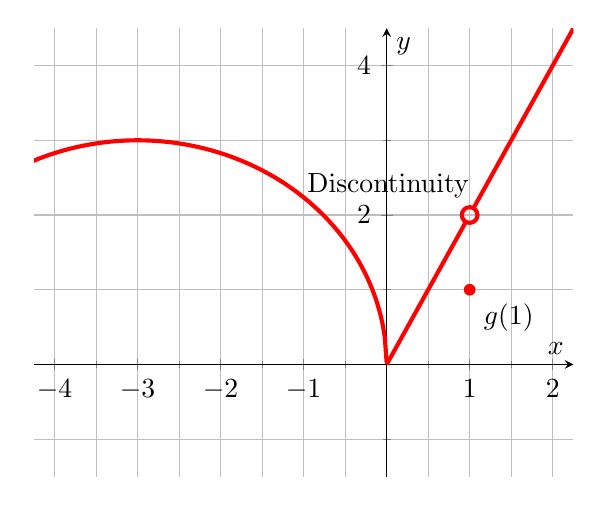
\begin{tikzpicture}
      \begin{axis}[
        axis lines = center,
        grid = both,
        xlabel={$x$},
        ylabel={$y$},
        ymin=-1.5,
        ymax=4.5,
        xmax=2.25,
        xmin=-4.25,
        minor tick num = 1
      ]

        \addplot[line width=1.5pt, red, samples=200, domain=1.05:2.5]{2*x};
        \addplot[line width=1.5pt, red, samples=200, domain=0:.95]{2*x};
        \addplot[line width=1.5pt, red, samples=200, domain=-4.5:-0.0001]{sqrt(9-(x+3)^2)};

        \node[red, circle, draw, inner sep=2pt, line width=1.5pt, label={[xshift=0.2cm]above left: Discontinuity}] at (axis cs: 1, 2) {};
        \node[red, circle, fill, inner sep=1.5pt, label={below right: $g(1)$}] at (axis cs: 1, 1) {};
      \end{axis}
    \end{tikzpicture}
  \end{minipage}
\end{questions}
\end{document}
